% !TEX TS-program = pdflatex
% !TEX encoding = UTF-8 Unicode

\documentclass[11pt]{report} % use larger type; default would be 10pt

\usepackage[utf8]{inputenc} % set input encoding (not needed with XeLaTeX)

\usepackage{listings} % source code formatting
\usepackage{hyperref}
%%% Examples of Article customizations
% These packages are optional, depending whether you want the features they provide.
% See the LaTeX Companion or other references for full information.

%%% PAGE DIMENSIONS
\usepackage{geometry} % to change the page dimensions
\geometry{a4paper} % or letterpaper (US) or a5paper or....
% \geometry{margin=2in} % for example, change the margins to 2 inches all round
% \geometry{landscape} % set up the page for landscape
%   read geometry.pdf for detailed page layout information

\usepackage{graphicx} % support the \includegraphics command and options

% \usepackage[parfill]{parskip} % Activate to begin paragraphs with an empty line rather than an indent

%%% PACKAGES
\usepackage{booktabs} % for much better looking tables
\usepackage{array} % for better arrays (eg matrices) in maths
\usepackage{paralist} % very flexible & customisable lists (eg. itemize/itemize, etc.)
\usepackage{verbatim} % adds environment for commenting out blocks of text & for better verbatim
\usepackage{subfig} % make it possible to include more than one captioned figure/table in a single float
% These packages are all incorporated in the memoir class to one degree or another...

%%% HEADERS & FOOTERS
\usepackage{fancyhdr} % This should be set AFTER setting up the page geometry
\pagestyle{fancy} % options: empty , plain , fancy
\renewcommand{\headrulewidth}{0pt} % customise the layout...
\lhead{Links - Project Report}\chead{}\rhead{}
\lfoot{}\cfoot{\thepage}\rfoot{}

%%% SECTION TITLE APPEARANCE
\usepackage{sectsty}
\allsectionsfont{\sffamily\mdseries\upshape} % (See the fntguide.pdf for font help)
% (This matches ConTeXt defaults)

%%% ToC (table of contents) APPEARANCE
\usepackage[nottoc,notlof,notlot]{tocbibind} % Put the bibliography in the ToC
\usepackage[titles,subfigure]{tocloft} % Alter the style of the Table of Contents
\renewcommand{\cftsecfont}{\rmfamily\mdseries\upshape}
\renewcommand{\cftsecpagefont}{\rmfamily\mdseries\upshape} % No bold!
\renewcommand{\chaptername}{}

\usepackage{titlesec}
\usepackage{lipsum}
\titleformat{\chapter}
{\filcenter\normalfont\LARGE\bfseries}
{\chaptertitlename~\thechapter} {0.5em} {}


%%% END Article customizations

%%% The "real" document content comes below...

\title{Links - Project Report}
\author{Abhijith Madhav, Arjun S Bharadwaj}
%\date{} % Activate to display a given date or no date (if empty),
         % otherwise the current date is printed 

\begin{document}
\maketitle

\tableofcontents
\chapter{Introduction}

A bookmarking service is a centralized online service which enables users to add, annotate, edit and share bookmarks of web document.,The most popular bookmarking service currently is \emph{Delicious}. \emph{Scuttle} is one of the other well known open source alternative. 


\emph {Links} is envisioned as a similer online bookmarking service with the specific requirement that it should be deployable on a private server within an organization. The purpose is to enable people in an organization to share bookmarks with each other.



\emph {Links} is intended to be an extensible, modular system with an exposed API. Third parties must be able to write plugins and applications using this API.


It is envisioned to seemlessly fit into the share motto of the net community, be it through simple email or through popular social platforms like facebook and twitter.



\chapter{Requirements Specification}
\section{Functional Requirements}
This section provides the functional requirements of the project.
\begin{enumerate}
	\item
		Login
		\begin{itemize}
			\item
				User logs into the system.
			\item
				\emph{Input:} User enters the login details and clicks on login.
			\item
				\emph{Output:} 
					\begin{itemize}
						\item
							If the validation of the user credentials is successful:
							\begin{itemize}
								\item
									The user is redirected to the Homepage.
							\end{itemize}


						\item
							If the validation of the login details is unsuccessful:
							\begin{itemize}
								\item
									An appropriate error message is shown to the user.
							\end{itemize}
					\end{itemize}
		\end{itemize}

	\item
		Signup
		\begin{itemize}
			\item
				User clicks on Signup.
			\item
				\emph{Input:} Signup details are asked.
			\item
				\emph{Output:} 
					\begin{itemize}
						\item	
							If validation of the details is successful:
							\begin{itemize}
								\item
									Account is created.
							\end{itemize}

						\item
							If validation of the details is unsuccessful:
							\begin{itemize}
								\item
									An appropriate error message is shown to the user.
							\end{itemize}
					\end{itemize}
		\end{itemize}

	\item
		Save Links
		\begin{itemize}
			\item
				User bookmarks the links.
			\item
				\emph{Input:} A Title, URI, Tags and Annotations are provided.
			\item
				\emph{Output:} 
					\begin{itemize}
						\item				
							After the link is saved:
							\begin{itemize}
								\item
									Acknowledgement for the action is provided.
									\item
									Suggest tags if same link was shared by others based on the visibility level of the user.
							\end{itemize}			
					\end{itemize}					
		\end{itemize}

	\item
		Edit  Links
		\begin{itemize}
			\item
				User edits the links.
			\item
				\emph{Input:} An existing link, modified data (title, tags, annotations).
			\item
				\emph{Output:} 
					\begin{itemize}
						\item	
							After the link is updated:
						\begin{itemize}
							\item
								Acknowledgement for the update is provided.
						\end{itemize}						
					\end{itemize}			
		\end{itemize}


	\item
		Delete   Links
		\begin{itemize}
			\item
				User deletes  the links.
			\item
				\emph{Input:} An existing link shared by the user.
			\item
				\emph{Output:} 
					\begin{itemize}
						\item	
							After the link is deleted:
						\begin{itemize}
							\item
								Acknowledgement for the deletion is provided.
						\end{itemize}			
					\end{itemize}
			\end{itemize}

	\item
		Create User Groups
		\begin{itemize}
			\item
				Creation of Groups by the user.
			\item
				\emph{Input:} Group name and group description corresponding to the group.
			\item
				\emph{Output:} 
					\begin{itemize}
						\item
							If the group name is not already used:
						\begin{itemize}
							\item
								Acknowledgement for the creation is provided.
						\end{itemize}

						\item
							If the group name already exists:
						\begin{itemize}
							\item
								Appropriate error message.
						\end{itemize}
					\end{itemize}			
			\end{itemize}

	\item
		Join Group
		\begin{itemize}
			\item
				User joins the group.
			\item
				\emph{Input:} Group name of the group that the user wishes to subscribe to.
			\item
				\emph{Output:} Acknowledgement of the subscription is provided.
		\end{itemize}

	\item
		Unjoin Group
		\begin{itemize}
			\item
				User unjoins the group.
			\item
				\emph{Input:} Group name of the group that the user wishes to unsubscribe to.
			\item
				\emph{Output:} Acknowledgement of the un-subscription is provided.
		\end{itemize}

	\item
		Share
		\begin{itemize}
			\item
				Sharing of the links.
			\item
				\emph{Input:} A set of bookmarks to be shared via email or popular social media
			\item
				\emph{Output:} Share bookmarks via the specified media.
		\end{itemize}

	\item
		Add Members
		\begin{itemize}
			\item
				Add members to the group.
			\item
				\emph{Input:} User names by the group owner.
			\item
				\emph{Output:} Acknowledgement of addition to group.
		\end{itemize}


	\item
		Remove Members
		\begin{itemize}
			\item
				Remove members to the group.
			\item
				\emph{Input:} User names by the group owner.
			\item
				\emph{Output:} Acknowledgement of deletion to group.
		\end{itemize}
\item
Interoperability\\
Expose APIs through which the following can be done
\begin{itemize}
\item
Search based on bookmarks, annotations, tags in accordance to the visibility of the user.
\item
Add, delete and edit the bookmarks in accordance to the visibility of the user.
\end{itemize}
As a proof of concept, an android application that consumes the data from the provided APIs will be created
\end{enumerate}
\maketitle
\section{Non-functional Requirements}
\subsection{Security Requirements}
\begin{enumerate}
\item
All users must be authenticated before being given modification privileges in “Links”.
\item
Third party clients must not have access to passwords of users and must instead use a token based authentication scheme.
\item
User passwords must be stored as salted hashes in the "Links" system.
\item
HTTPS connections between clients and the "Links" server must be supported.
\end{enumerate}
\subsection{User Experience}
\begin{enumerate}
\item
The browser extension using the "Links" API  must enable saving and/or sharing bookmarks from a third party website without having to navigate away from that site.
\item
Where possible, portions of any "Links" webpage must be updated without having to refresh the entire webpage from the server.
\end{enumerate}


\chapter{Architecture and Design}

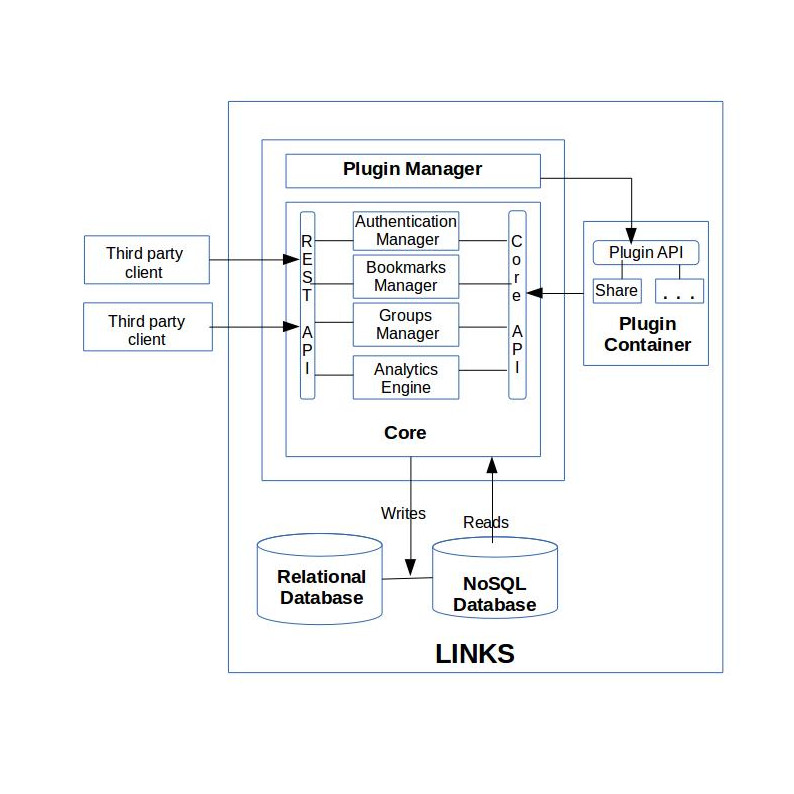
\includegraphics[scale=0.5]{architecture_diagram.jpg}
\section{Architechture}
The architechture of 'Links' consists mainly of a core module providing the basic functionality of storing, retrieving and sharing of bookmarks. The proposed architecture also has an analytics engine as a part of the core which is yet to be implemented.

The plugin module is intended to help extend a 'Links' installation by 'plugging in' useful functionalities. It consists of a plugin manager which loads at launch time all the small self contained plugins into 'Links'.

\subsection{Core Module}
The core consists of an authentication manager, bookmarks manager and a groups manager which implement functionality required for authentication, bookmarks management, groups management and sharing of bookmarks through groups.

\subsection{Plugin Module}
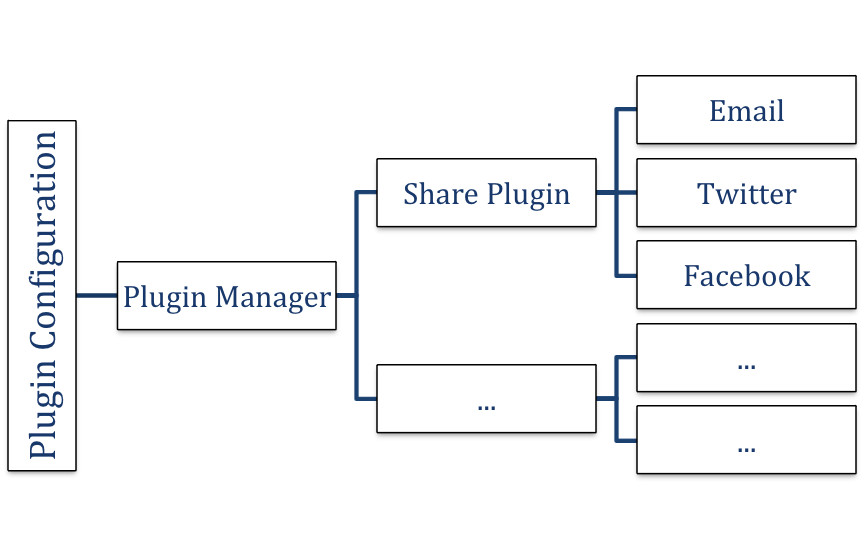
\includegraphics[scale=.5]{PluginArchitecture.png}

These are the components of the Plugin Module.
\begin{enumerate}

\item
	Configuration File: This file will consist of all the plugins that are enabled in the system.
\item
	Plugin Manager: The Plugin Manager will lookup the configuration file and will enable/disale the plugins.
\item
	Share Plugin: This is a sample plugin implemented which will help to share the links on various platforms like Email, Twitter and Facebook.
\end{enumerate}
\section{Database Design}
The core of Links access the database for data persistance. The class diagram detailing the schema and relationships is as follows

\includegraphics[scale=0.3]{Datamodel.png}

\chapter{Implementation}

\section{Technology used}
\begin{itemize}
\item
A MySQL instance is used for the database because of previous familiarity  with the same.
\item
Ruby on Rails is used as the web application framework. The reasons for the same are
\begin{itemize}
\item
A full-stack framework that emphasizes the use of well-known software engineering patterns and paradigms, including convention over configuration (CoC), the active record pattern, and model–view–controller (MVC).
\item
Easy to plugin gems to implement many common features of web application.
\item
Faster development time.
\end{itemize}
\end{itemize}

\section{Controllers}
The functionality of The core module is realized by implementing controllers in the rails MVC  framework. The implemented controllers can be found at /links/links/app/controllers. The main ones are briefly described below.
\begin{itemize}
\item
bookmarks\textunderscore controller.rb : Implements methods to perform create, update and delete operations on the bookmarks object.
\item
groups\textunderscore controller.rb : Implements methods to perform create, update and delete operations on the groups object.
\item
searches\textunderscore controller.rb : Implements methods to perfom retrieve operations on the bookmarks and groups objects.
pages\textunderscore controller.rb : Implements simple methods to render static pages.
\end{itemize}

\section{Authentication and User Management}
Authentication into Links for a user is implemented using the Devise gem. Devise is a flexible authentication solution for Rails which takes care of the entire user management process and authentication process. Features not available by default in Devise can easily be added and are added in users\textunderscore controller.rb. Uploading the photo of the user and display of the same is added in this way.

\section{Authorization and REST API's}
API's to perform CRUD operations on bookmark and group objects are exposed in a RESTFUL way. Controllers for same can be found in /links/links/app/controllers/api/v1.

Authorization for third party clients is through OAuth2 protocol. Doorkeeper gem is used to implement a OAuth provider inside of Links.

Documentation for obtaining authorization and usage of the RESTful API's can be found  \href{https://bitbucket.org/linkiiitb/links/wiki/Links\%20API\%20documentation}{here}.

\section{Import from Delicious}
This is a feature which helps in migration of bookmarks from Delicious. delicious\textunderscore controller.rb implements an OAuth client which pulls a users bookmarks from his Delicious account and integrates the same with his Links account. It is intended to make this as a plugin rather than as a core feature in future.

\chapter{Future work}
The following are the features that need to be worked on
\begin{itemize}
\item
Analytics Engine and tags suggestions.
\item
A more sophisticated installation script.
\item
Admin UI specifically to administer plugins.
\item
Make the import feature as a plugin.
\end{itemize}
\end{document}
